% !TeX root = document.tex
% !TeX encoding = UTF-8 Unicode

\chapter*{Introdução e Contextualização}%
\label{introducao}

MPC é uma técnica de controle avançada que utiliza o modelo do sistema para
prever a saída em momentos futuros e, com isso, gerar uma estratégia de
controle. Para isso é utilizado o conceito de controle por horizonte recessivo,
onde a o sinal de ótimo controle é planejado para os próximos \(N_c\) instantes,
mas apenas o primeiro é utilizado, recalculando-se toda a estratégia no instante
seguinte, de forma a possibilitar a reação à possíveis distúrbios.

Algumas vantagens desta técnica é que os conceitos utilizados são simples e
fáceis de serem transformados em módulos reutilizáveis, além de ser possível
utilizar a técnica tanto para gerar controladores primários, que atuam
diretamente no sistema, quanto supervisórios, que gerenciam um conjunto de
controladores mais baixos na hierarquia. Sua principal vantagem, no entanto, é
que pode-se modelar restrições físicas, como saturação de entrada e saída ou
taxa de modificação destas grandezas, diretamente no controlador
(\textcite{book:wang}).

Por exemplo, a inserção das restrições na variável de controle no modelo do
controlador torna a resposta diferente da resposta gerada por controladores onde
a restrição é imposta após a geração do sinal de controle, sem que o controlador
tome ciência da mesma. Com a restrição exógena, como quando se usa a técnica de
\textit{anti-windup}, o controlador continua gerando sinais de controle que irão
saturar e não irão, de fato, alterar a resposta além deste limite físico. Quando
o modelo tem ciência desta limitação, no entanto, ele tende a gerar sinais de
controle que irão fazer o melhor o possível dentro da faixa de saturação, até
mesmo trabalhando com a mesma, mas de forma mais \enquote{consciente}, que
dizer, sabendo que o atuador está saturado.

Normalmente utiliza-se sistemas a parâmetros concentrados (SPC) para modelar
sistemas físicos. Nesses sistemas as variáveis de interesse se alteram apenas no
domínio do tempo. Em sistemas a parâmetros distribuídos (SPD), no entanto, a
variável de interesse também depende do espaço. Tais sistemas são normalmente
representados por equações diferenciais parciais
(\textcite{masterthesis:nelson}).

Tomando o forno do Laboratório de Sinais e Sistemas como exemplo podemos ver na
Figura~\ref{fig:sensors-spd} os sensores \(S_1\) a \(S_5\) e o fluxo de ar
quente q. Imagine que queiramos controlar a temperatura na posição onde
encontra-se o sensor \(S_3\), mas que apenas o sensor \(S_5\) esteja
funcionando. Com um modelo SPD podemos ter dois modelos SPC\@: um que modele o
fluxo de temperatura até o sensor \(S_3\) e um outro que modele de \(S_3\) até
\(S_5\), ambos interconectados. Desta forma podemos utilizar um observador e a
leitura do sensor \(S_5\) para estimar a temperatura no sensor \(S_3\), e
controlá-la mesmo sem fazer sua medição direta.

\begin{figure}[ht!]
    \centering
    \captionsetup{justification=centering}
    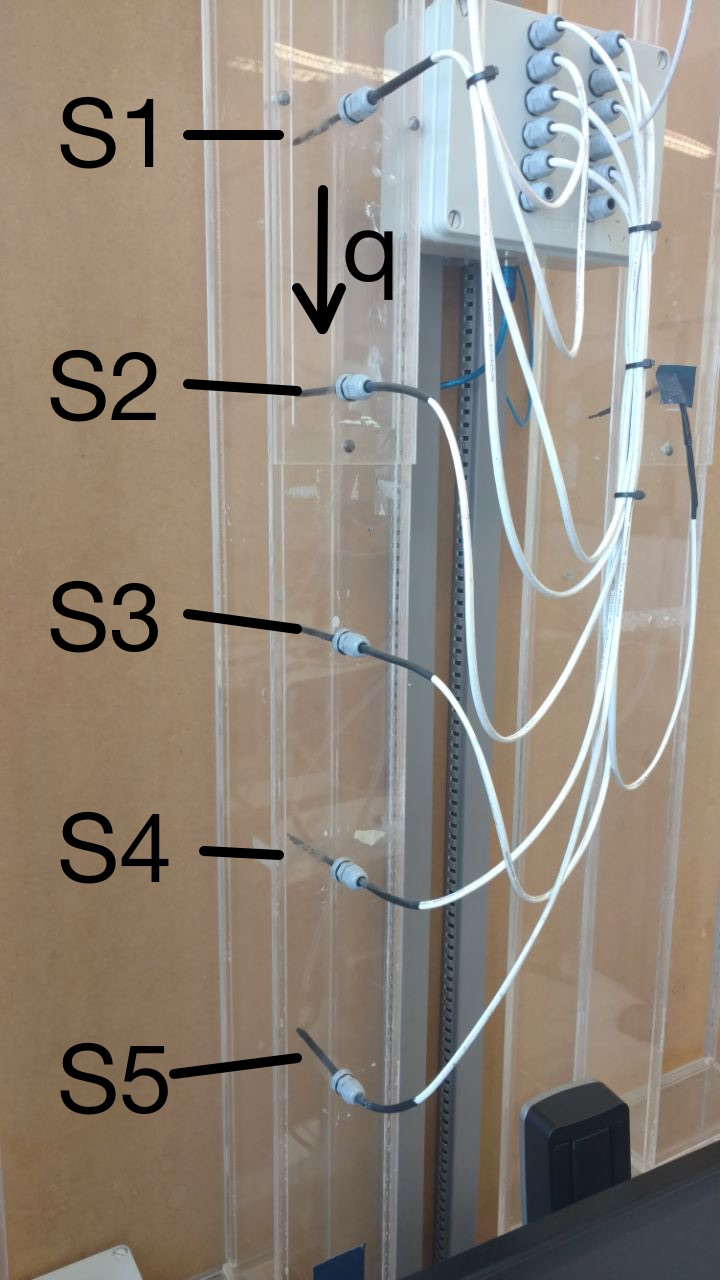
\includegraphics[height=0.5\linewidth]{imgs/planta-spd}
    \caption{Sensores da planta}%
    \label{fig:sensors-spd}
\end{figure}

O observador é um sistema que estima os estados de um modelo baseado nas
entradas e saídas do mesmo. O observador de Kalman, também conhecido como filtro
de Kalman, é uma formulação que permite estimar o modelo de forma precisa mesmo
na presenta de ruídos, seja na leitura da saída ou dos próprios estados.

O uso de controladores MPC com modelos SPD não é novo. Sua maior aplicação, no
entanto, continua sendo na área da química e fabricação de aço. Assim esta
proposta visa o desenvolvimento de um controlador que utiliza técnicas
conhecidas de uma maneira não convencional. Espera-se com isto mostrar a
eficiência desta combinação (\textcite{article:shang}).

Em ambientes industriais é comum o uso de computadores lógicos programáveis para
fazer a interface com o hardware. No meio acadêmico, no entanto, utiliza-se
softwares como o \textit{MATLAB} e \textit{LabVIEW} para a prototipagem rápida.
Isto requer que o pesquisador recrie a interface gráfica e controle a aquisição
de dados manualmente, o que consome tempo que poderia ser gasto com a pesquisa.

Assim, uma plataforma que faça a interface com o hardware e possibilite a
execução de um controlador de forma transparente permite que o pesquisador se
concentre nestes estudos e não se preocupe com detalhes da implementação da
aquisição dos dados. Tal ferramenta também permitiria ao pesquisador
interagir com CLPs, desenvolvendo e testando controladores de forma fácil em
uma linguagem simples (Python) sem se preocupar com todas as nuâncias das
linguagens LADDER utilizadas nos PLCs, podendo implementar seu controlador nesta
linguagem limitada apenas ao final, quando este tiver sido devidamente testado.

A aplicação de uma plataforma para controle em todos as plantas do laboratório
permite que os usuários possam migrar de uma planta para outra sem dificuldades.
Também permite que controladores e observadores desenvolvidos sejam testados em
diferentes plantas com poucas modificações, já que as interfaces seriam as
mesmas em todas elas.

\noindent
{\textbf Áreas envolvidas}

A principal área deste trabalho é controle, por ter o maior peso teórico e de
desenvolvimento. No entanto o trabalho também contempla as áreas de elétrica,
pelas modificações que serão feitas na eletrônica de acionamento e aquisição de
dados do forno, e computação, pelas modificações que serão feitas na plataforma
de controle para que esta possa se comunicar com o hardware e as modificações
que serão feitas para corrigir defeitos e implementar melhorias, como, por
exemplo, recuperar o erro do banco de dados e exibir para o usuário e, caso
possível, gerar mensagens de erro mais informativas, que apontam o lugar do
erro.
